\ifdefined\GlandersWatchReport
\else
\documentclass[tikz,border=10pt]{standalone}
\usepackage[T1]{fontenc}
\usepackage[scaled=0.95]{helvet}
\renewcommand{\familydefault}{\sfdefault}
\usepackage{xcolor}
\usetikzlibrary{arrows.meta,calc}
\fi

\definecolor{gwnavy}{HTML}{1F3A5F}
\definecolor{gwamber}{HTML}{B45309}
\definecolor{gwgreen}{HTML}{15803D}
\definecolor{gwslate}{HTML}{475569}
\definecolor{gwviolet}{HTML}{6D28D9}
\definecolor{gwblue}{HTML}{1D4ED8}
\definecolor{gwteal}{HTML}{0F766E}

\tikzset{
  box/.style={draw=#1!75!black, fill=#1!7, rounded corners=3pt, line width=0.8pt, align=left, font=\scriptsize},
  flow/.style={-{Stealth[length=2.6mm,width=2mm]}, line width=1.1pt, gwnavy},
  plug/.style={-{Stealth[length=2.4mm,width=1.8mm]}, dashed, line width=0.9pt, gwslate},
  lbl/.style={font=\tiny\bfseries, text=gwnavy, fill=white, inner sep=1.2pt},
  port/.style={circle, draw=gwviolet!80!black, fill=gwviolet!25, line width=0.9pt, minimum size=0.42cm, inner sep=0pt},
  chip/.style={draw=gwgreen!70!black, fill=gwgreen!12, rounded corners=2pt, line width=0.7pt, font=\scriptsize, align=center, inner sep=3pt},
  chipx/.style={draw=gwslate!80, fill=white, dashed, rounded corners=2pt, line width=0.8pt, font=\scriptsize, align=center, inner sep=3pt},
}
\newcommand{\blk}[8]{%
  \pgfmathsetlengthmacro{\bw}{(#5-#3)*1cm}%
  \pgfmathsetlengthmacro{\bh}{(#6-#4)*1cm}%
  \pgfmathsetlengthmacro{\tw}{(#5-#3)*1cm-10pt}%
  \node[box=#2,#7,anchor=south west,minimum width=\bw,minimum height=\bh,text width=\tw,inner sep=5pt](#1) at (#3,#4){#8};}
\newcommand{\cont}[7]{%
  \draw[draw=#1!70!black, fill=#1!4, rounded corners=5pt, line width=1pt, #7] (#2,#3) rectangle (#4,#5);
  \node[anchor=north west, font=\small\bfseries, text=#1!60!black] at (#2+0.2,#5-0.1) {#6};}
\ifdefined\GlandersWatchReport
\else
\begin{document}
\fi
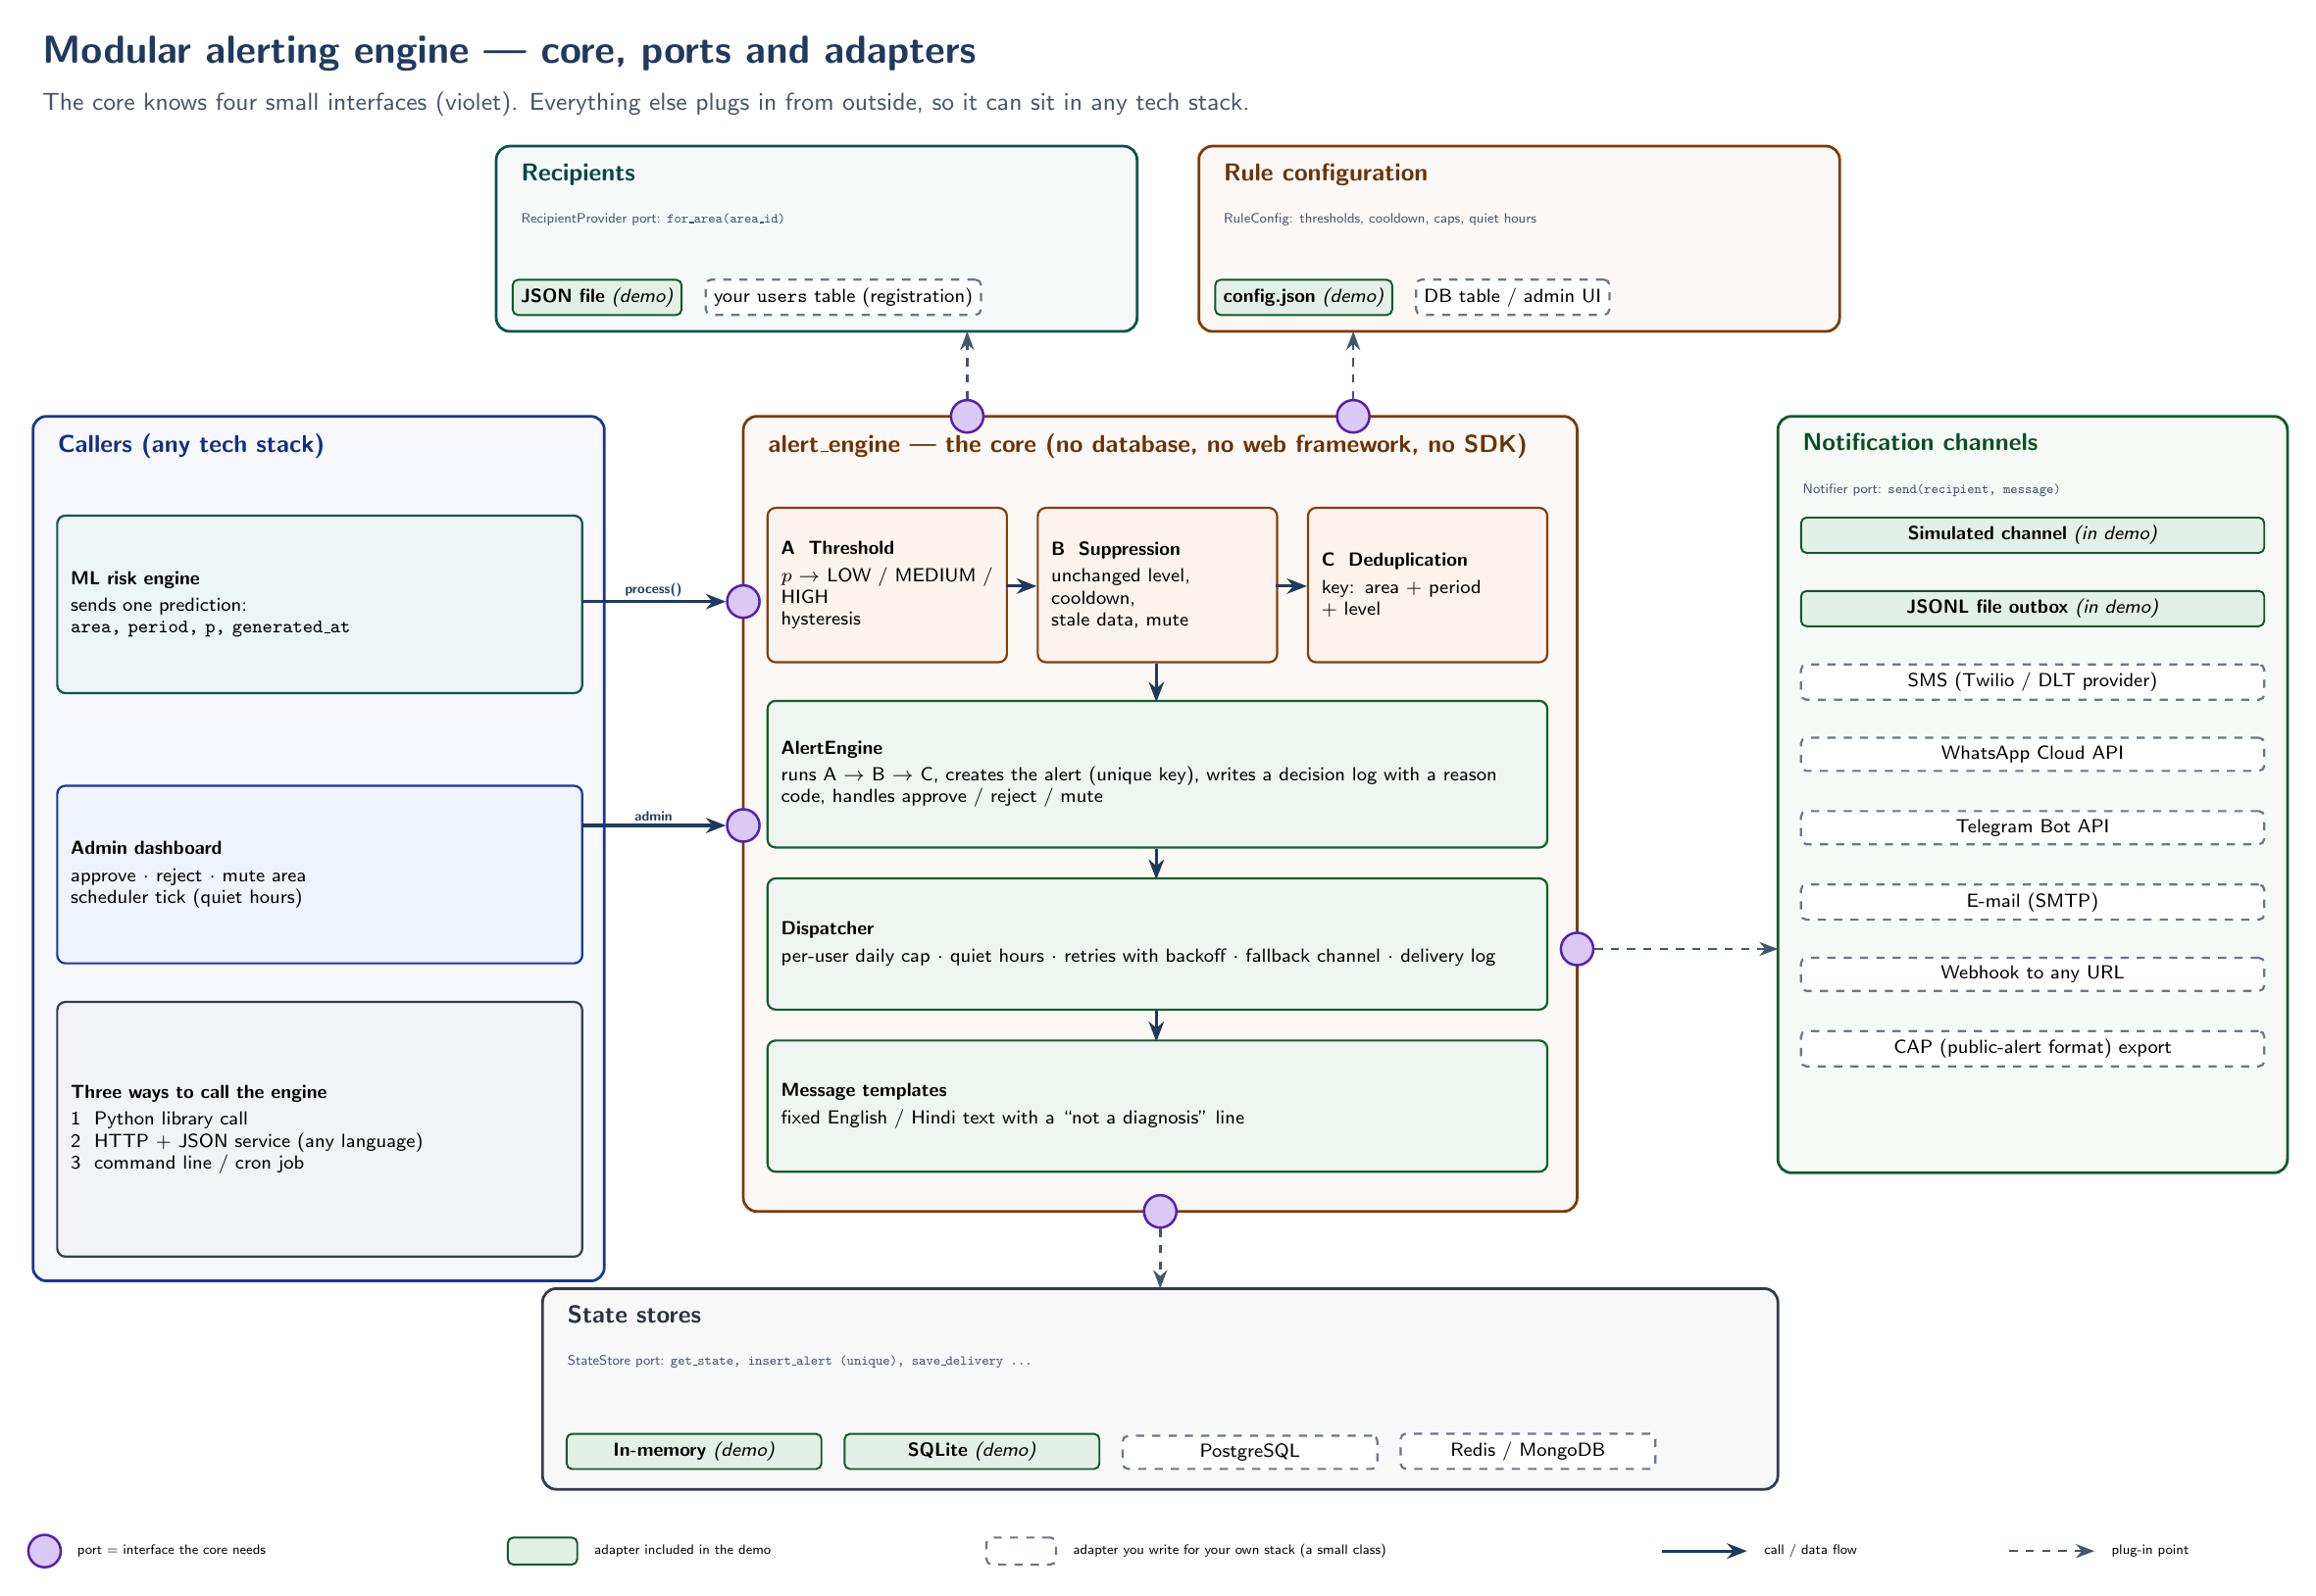
\begin{tikzpicture}[x=1cm,y=1cm]

\node[anchor=west, font=\Large\bfseries, text=gwnavy] at (0.4,18.9) {Modular alerting engine --- core, ports and adapters};
\node[anchor=west, font=\small, text=gwslate] at (0.4,18.25) {The core knows four small interfaces (violet). Everything else plugs in from outside, so it can sit in any tech stack.};

% ============ CALLERS (left) ============
\cont{gwblue}{0.4}{3.0}{7.8}{14.2}{Callers (any tech stack)}{}
\blk{ml}{gwteal}{0.7}{10.6}{7.5}{12.9}{}{\textbf{ML risk engine}\\[2pt]sends one prediction:\\ \texttt{area, period, p, generated\_at}}
\blk{adm}{gwblue}{0.7}{7.1}{7.5}{9.4}{}{\textbf{Admin dashboard}\\[2pt]approve $\cdot$ reject $\cdot$ mute area\\ scheduler tick (quiet hours)}
\blk{ways}{gwslate}{0.7}{3.3}{7.5}{6.6}{}{\textbf{Three ways to call the engine}\\[2pt]
1\ \ Python library call\\
2\ \ HTTP + JSON service (any language)\\
3\ \ command line / cron job}

% ============ CORE ============
\cont{gwamber}{9.6}{3.9}{20.4}{14.2}{alert\_engine --- the core (no database, no web framework, no SDK)}{}
\blk{sA}{gwamber}{9.9}{11.0}{13.0}{13.0}{}{\textbf{A\ \ Threshold}\\[2pt]$p \rightarrow$ LOW / MEDIUM / HIGH\\hysteresis}
\blk{sB}{gwamber}{13.4}{11.0}{16.5}{13.0}{}{\textbf{B\ \ Suppression}\\[2pt]unchanged level, cooldown,\\stale data, mute}
\blk{sC}{gwamber}{16.9}{11.0}{20.0}{13.0}{}{\textbf{C\ \ Deduplication}\\[2pt]key: area + period\\+ level}
\draw[flow] (13.0,12.0) -- (13.4,12.0);
\draw[flow] (16.5,12.0) -- (16.9,12.0);
\blk{eng}{gwgreen}{9.9}{8.6}{20.0}{10.5}{}{\textbf{AlertEngine}\\[2pt]runs A $\rightarrow$ B $\rightarrow$ C, creates the alert (unique key), writes a decision log with a reason code, handles approve / reject / mute}
\blk{dis}{gwgreen}{9.9}{6.5}{20.0}{8.2}{}{\textbf{Dispatcher}\\[2pt]per-user daily cap $\cdot$ quiet hours $\cdot$ retries with backoff $\cdot$ fallback channel $\cdot$ delivery log}
\blk{tpl}{gwgreen}{9.9}{4.4}{20.0}{6.1}{}{\textbf{Message templates}\\[2pt]fixed English / Hindi text with a ``not a diagnosis'' line}
\draw[flow] (14.95,11.0) -- (14.95,10.5);
\draw[flow] (14.95,8.6) -- (14.95,8.2);
\draw[flow] (14.95,6.5) -- (14.95,6.1);

% ============ PORTS ============
\node[port] (pin) at (9.6,11.8) {};
\node[port] (padm) at (9.6,8.9) {};
\node[port] (pnot) at (20.4,7.3) {};
\node[port] (pst) at (15.0,3.9) {};
\node[port] (prec) at (12.5,14.2) {};
\node[port] (pcfg) at (17.5,14.2) {};

% callers -> ports
\draw[flow] (7.5,11.8) -- (pin.west) node[pos=0.5,above,lbl]{process()};
\draw[flow] (7.5,8.9) -- (padm.west) node[pos=0.5,above,lbl]{admin};

% ============ ADAPTERS: channels (right) ============
\cont{gwgreen}{23.0}{4.4}{29.6}{14.2}{Notification channels}{}
\node[font=\tiny, text=gwslate, anchor=north west] at (23.2,13.45) {Notifier port: \texttt{send(recipient, message)}};
\node[chip, minimum width=6.0cm, anchor=north] at (26.3,12.9) {\textbf{Simulated channel} \textit{(in demo)}};
\node[chip, minimum width=6.0cm, anchor=north] at (26.3,11.95) {\textbf{JSONL file outbox} \textit{(in demo)}};
\node[chipx, minimum width=6.0cm, anchor=north] at (26.3,11.0) {SMS (Twilio / DLT provider)};
\node[chipx, minimum width=6.0cm, anchor=north] at (26.3,10.05) {WhatsApp Cloud API};
\node[chipx, minimum width=6.0cm, anchor=north] at (26.3,9.1) {Telegram Bot API};
\node[chipx, minimum width=6.0cm, anchor=north] at (26.3,8.15) {E-mail (SMTP)};
\node[chipx, minimum width=6.0cm, anchor=north] at (26.3,7.2) {Webhook to any URL};
\node[chipx, minimum width=6.0cm, anchor=north] at (26.3,6.25) {CAP (public-alert format) export};
\draw[plug] (pnot.east) -- (23.0,7.3);

% ============ ADAPTERS: state stores (bottom) ============
\cont{gwslate}{7.0}{0.3}{23.0}{2.9}{State stores}{}
\node[font=\tiny, text=gwslate, anchor=north west] at (7.2,2.15) {StateStore port: \texttt{get\_state, insert\_alert (unique), save\_delivery ...}};
\node[chip, minimum width=3.3cm, anchor=south west] at (7.3,0.55) {\textbf{In-memory} \textit{(demo)}};
\node[chip, minimum width=3.3cm, anchor=south west] at (10.9,0.55) {\textbf{SQLite} \textit{(demo)}};
\node[chipx, minimum width=3.3cm, anchor=south west] at (14.5,0.55) {PostgreSQL};
\node[chipx, minimum width=3.3cm, anchor=south west] at (18.1,0.55) {Redis / MongoDB};
\draw[plug] (pst.south) -- (15.0,2.9);

% ============ ADAPTERS: recipients + config (top) ============
\cont{gwteal}{6.4}{15.3}{14.7}{17.7}{Recipients}{}
\node[font=\tiny, text=gwslate, anchor=north west] at (6.6,16.95) {RecipientProvider port: \texttt{for\_area(area\_id)}};
\node[chip, anchor=south west] at (6.6,15.5) {\textbf{JSON file} \textit{(demo)}};
\node[chipx, anchor=south west] at (9.1,15.5) {your \texttt{users} table (registration)};
\draw[plug] (prec.north) -- (12.5,15.3);

\cont{gwamber}{15.5}{15.3}{23.8}{17.7}{Rule configuration}{}
\node[font=\tiny, text=gwslate, anchor=north west] at (15.7,16.95) {RuleConfig: thresholds, cooldown, caps, quiet hours};
\node[chip, anchor=south west] at (15.7,15.5) {\textbf{config.json} \textit{(demo)}};
\node[chipx, anchor=south west] at (18.3,15.5) {DB table / admin UI};
\draw[plug] (pcfg.north) -- (17.5,15.3);

% ============ LEGEND ============
\node[port] at (0.55,-0.5) {};
\node[anchor=west, font=\tiny] at (0.85,-0.5) {port = interface the core needs};
\node[chip, minimum width=0.9cm, minimum height=0.35cm] at (7.0,-0.5) {};
\node[anchor=west, font=\tiny] at (7.55,-0.5) {adapter included in the demo};
\node[chipx, minimum width=0.9cm, minimum height=0.35cm] at (13.2,-0.5) {};
\node[anchor=west, font=\tiny] at (13.75,-0.5) {adapter you write for your own stack (a small class)};
\draw[flow] (21.5,-0.5) -- (22.6,-0.5);
\node[anchor=west, font=\tiny] at (22.7,-0.5) {call / data flow};
\draw[plug] (26.0,-0.5) -- (27.1,-0.5);
\node[anchor=west, font=\tiny] at (27.2,-0.5) {plug-in point};

\end{tikzpicture}
\ifdefined\GlandersWatchReport
\else
\end{document}
\fi